\documentclass[1p]{elsarticle_modified}
%\bibliographystyle{elsarticle-num}

%\usepackage[colorlinks]{hyperref}
%\usepackage{abbrmath_seonhwa} %\Abb, \Ascr, \Acal ,\Abf, \Afrak
\usepackage{amsfonts}
\usepackage{amssymb}
\usepackage{amsmath}
\usepackage{amsthm}
\usepackage{scalefnt}
\usepackage{amsbsy}
\usepackage{kotex}
\usepackage{caption}
\usepackage{subfig}
\usepackage{color}
\usepackage{graphicx}
\usepackage{xcolor} %% white, black, red, green, blue, cyan, magenta, yellow
\usepackage{float}
\usepackage{setspace}
\usepackage{hyperref}

\usepackage{tikz}
\usetikzlibrary{arrows}

\usepackage{multirow}
\usepackage{array} % fixed length table
\usepackage{hhline}

%%%%%%%%%%%%%%%%%%%%%
\makeatletter
\renewcommand*\env@matrix[1][\arraystretch]{%
	\edef\arraystretch{#1}%
	\hskip -\arraycolsep
	\let\@ifnextchar\new@ifnextchar
	\array{*\c@MaxMatrixCols c}}
\makeatother %https://tex.stackexchange.com/questions/14071/how-can-i-increase-the-line-spacing-in-a-matrix
%%%%%%%%%%%%%%%

\usepackage[normalem]{ulem}

\newcommand{\msout}[1]{\ifmmode\text{\sout{\ensuremath{#1}}}\else\sout{#1}\fi}
%SOURCE: \msout is \stkout macro in https://tex.stackexchange.com/questions/20609/strikeout-in-math-mode

\newcommand{\cancel}[1]{
	\ifmmode
	{\color{red}\msout{#1}}
	\else
	{\color{red}\sout{#1}}
	\fi
}

\newcommand{\add}[1]{
	{\color{blue}\uwave{#1}}
}

\newcommand{\replace}[2]{
	\ifmmode
	{\color{red}\msout{#1}}{\color{blue}\uwave{#2}}
	\else
	{\color{red}\sout{#1}}{\color{blue}\uwave{#2}}
	\fi
}

\newcommand{\Sol}{\mathcal{S}} %segment
\newcommand{\D}{D} %diagram
\newcommand{\A}{\mathcal{A}} %arc


%%%%%%%%%%%%%%%%%%%%%%%%%%%%%5 test

\def\sl{\operatorname{\textup{SL}}(2,\Cbb)}
\def\psl{\operatorname{\textup{PSL}}(2,\Cbb)}
\def\quan{\mkern 1mu \triangleright \mkern 1mu}

\theoremstyle{definition}
\newtheorem{thm}{Theorem}[section]
\newtheorem{prop}[thm]{Proposition}
\newtheorem{lem}[thm]{Lemma}
\newtheorem{ques}[thm]{Question}
\newtheorem{cor}[thm]{Corollary}
\newtheorem{defn}[thm]{Definition}
\newtheorem{exam}[thm]{Example}
\newtheorem{rmk}[thm]{Remark}
\newtheorem{alg}[thm]{Algorithm}

\newcommand{\I}{\sqrt{-1}}
\begin{document}

%\begin{frontmatter}
%
%\title{Boundary parabolic representations of knots up to 8 crossings}
%
%%% Group authors per affiliation:
%\author{Yunhi Cho} 
%\address{Department of Mathematics, University of Seoul, Seoul, Korea}
%\ead{yhcho@uos.ac.kr}
%
%
%\author{Seonhwa Kim} %\fnref{s_kim}}
%\address{Center for Geometry and Physics, Institute for Basic Science, Pohang, 37673, Korea}
%\ead{ryeona17@ibs.re.kr}
%
%\author{Hyuk Kim}
%\address{Department of Mathematical Sciences, Seoul National University, Seoul 08826, Korea}
%\ead{hyukkim@snu.ac.kr}
%
%\author{Seokbeom Yoon}
%\address{Department of Mathematical Sciences, Seoul National University, Seoul, 08826,  Korea}
%\ead{sbyoon15@snu.ac.kr}
%
%\begin{abstract}
%We find all boundary parabolic representation of knots up to 8 crossings.
%
%\end{abstract}
%\begin{keyword}
%    \MSC[2010] 57M25 
%\end{keyword}
%
%\end{frontmatter}

%\linenumbers
%\tableofcontents
%
\newcommand\colored[1]{\textcolor{white}{\rule[-0.35ex]{0.8em}{1.4ex}}\kern-0.8em\color{red} #1}%
%\newcommand\colored[1]{\textcolor{white}{ #1}\kern-2.17ex	\textcolor{white}{ #1}\kern-1.81ex	\textcolor{white}{ #1}\kern-2.15ex\color{red}#1	}

{\Large $\underline{11a_{287}~(K11a_{287})}$}

\setlength{\tabcolsep}{10pt}
\renewcommand{\arraystretch}{1.6}
\vspace{1cm}\begin{tabular}{m{100pt}>{\centering\arraybackslash}m{274pt}}
\multirow{5}{120pt}{
	\centering
	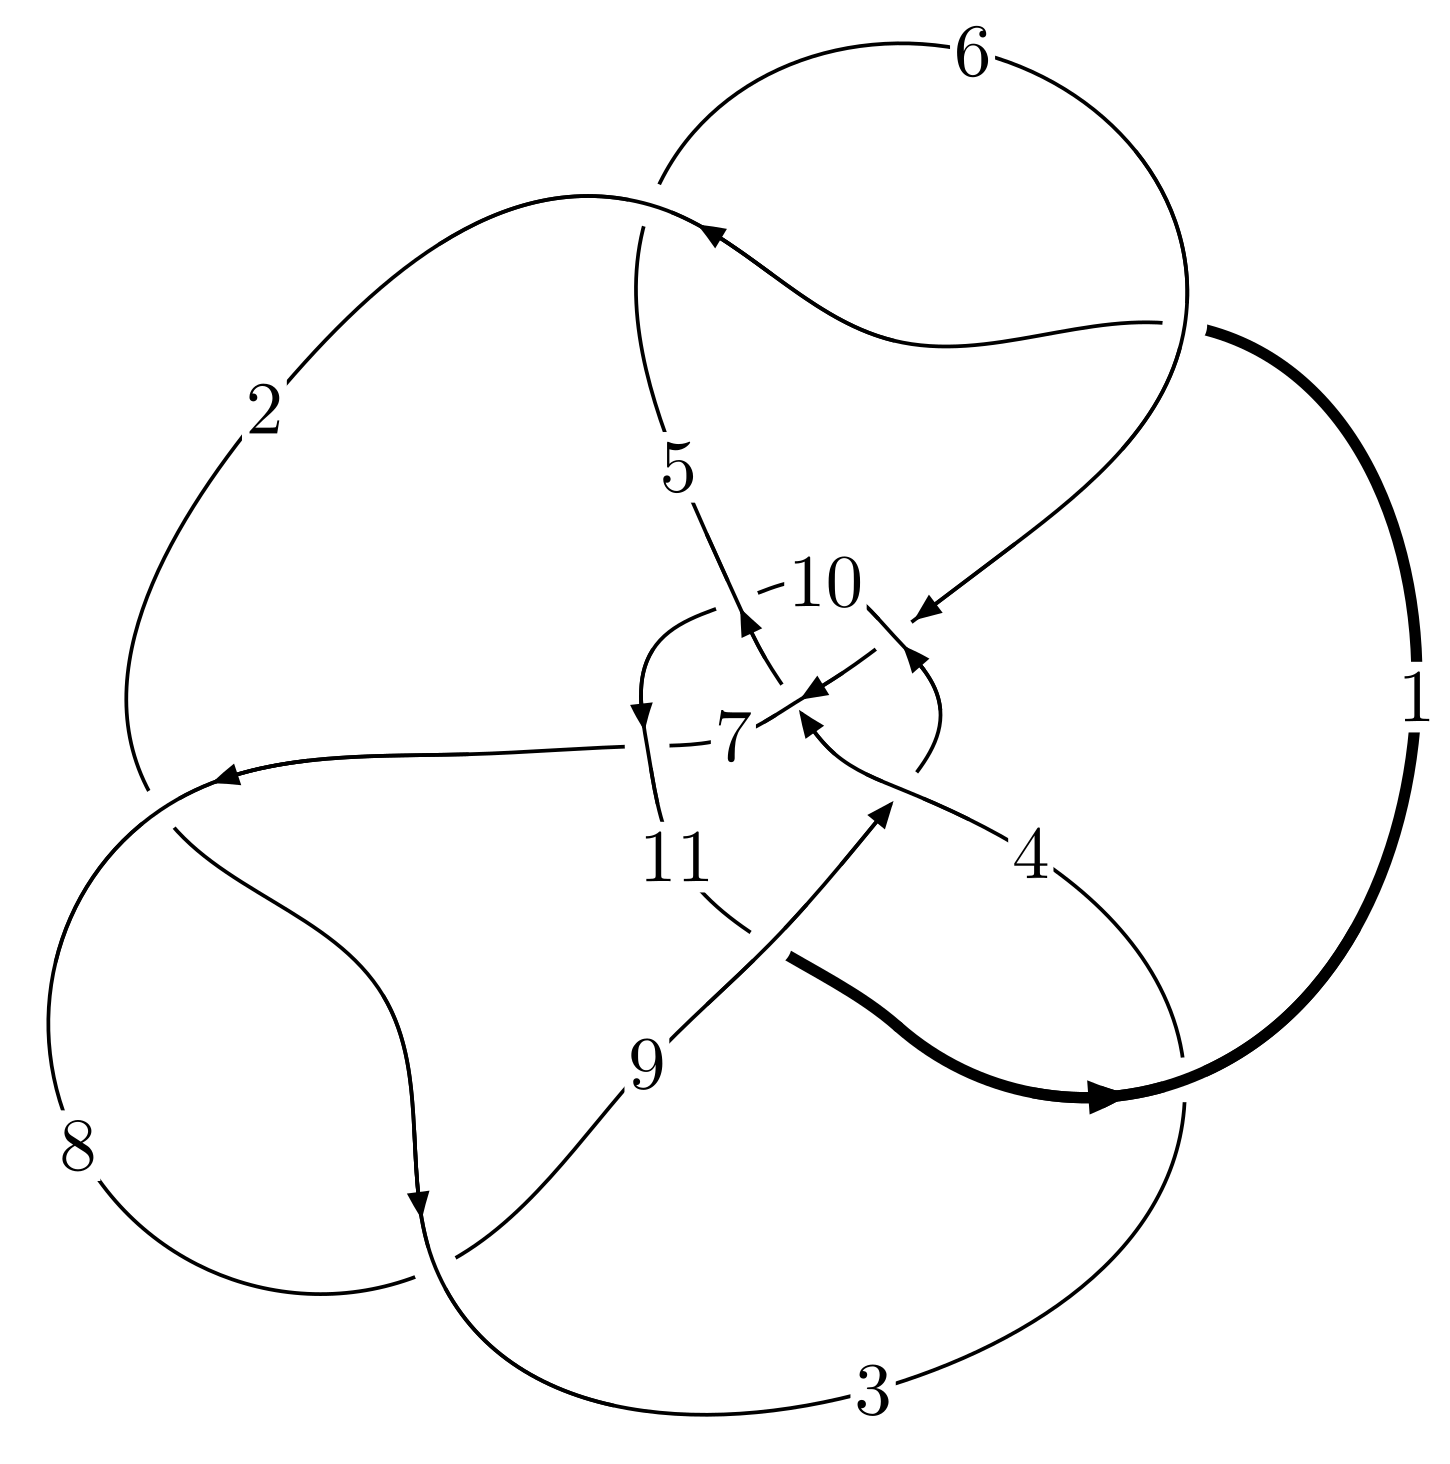
\includegraphics[width=112pt]{../../../GIT/diagram.site/Diagrams/png/536_11a_287.png}\\
\ \ \ A knot diagram\footnotemark}&
\allowdisplaybreaks
\textbf{Linearized knot diagam} \\
\cline{2-2}
 &
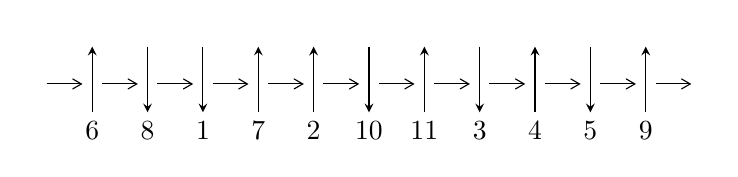
\begin{tikzpicture}[x=20pt, y=17pt]
	% nodes
	\node (C0) at (0, 0) {};
	\node (C1) at (1, 0) {};
	\node (C1U) at (1, +1) {};
	\node (C1D) at (1, -1) {6};

	\node (C2) at (2, 0) {};
	\node (C2U) at (2, +1) {};
	\node (C2D) at (2, -1) {8};

	\node (C3) at (3, 0) {};
	\node (C3U) at (3, +1) {};
	\node (C3D) at (3, -1) {1};

	\node (C4) at (4, 0) {};
	\node (C4U) at (4, +1) {};
	\node (C4D) at (4, -1) {7};

	\node (C5) at (5, 0) {};
	\node (C5U) at (5, +1) {};
	\node (C5D) at (5, -1) {2};

	\node (C6) at (6, 0) {};
	\node (C6U) at (6, +1) {};
	\node (C6D) at (6, -1) {10};

	\node (C7) at (7, 0) {};
	\node (C7U) at (7, +1) {};
	\node (C7D) at (7, -1) {11};

	\node (C8) at (8, 0) {};
	\node (C8U) at (8, +1) {};
	\node (C8D) at (8, -1) {3};

	\node (C9) at (9, 0) {};
	\node (C9U) at (9, +1) {};
	\node (C9D) at (9, -1) {4};

	\node (C10) at (10, 0) {};
	\node (C10U) at (10, +1) {};
	\node (C10D) at (10, -1) {5};

	\node (C11) at (11, 0) {};
	\node (C11U) at (11, +1) {};
	\node (C11D) at (11, -1) {9};
	\node (C12) at (12, 0) {};

	% arrows
	\draw[->,>={angle 60}]
	(C0) edge (C1) (C1) edge (C2) (C2) edge (C3) (C3) edge (C4) (C4) edge (C5) (C5) edge (C6) (C6) edge (C7) (C7) edge (C8) (C8) edge (C9) (C9) edge (C10) (C10) edge (C11) (C11) edge (C12) ;	\draw[->,>=stealth]
	(C1D) edge (C1U) (C2U) edge (C2D) (C3U) edge (C3D) (C4D) edge (C4U) (C5D) edge (C5U) (C6U) edge (C6D) (C7D) edge (C7U) (C8U) edge (C8D) (C9D) edge (C9U) (C10U) edge (C10D) (C11D) edge (C11U) ;
	\end{tikzpicture} \\
\hhline{~~} \\& 
\textbf{Solving Sequence} \\ \cline{2-2} 
 &
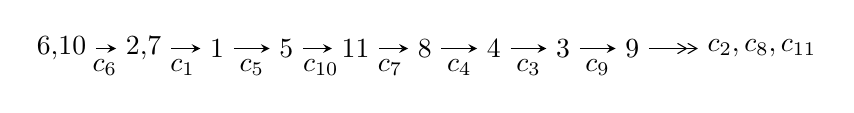
\begin{tikzpicture}[x=25pt, y=7pt]
	% node
	\node (A0) at (-1/8, 0) {6,10};
	\node (A1) at (17/16, 0) {2,7};
	\node (A2) at (17/8, 0) {1};
	\node (A3) at (25/8, 0) {5};
	\node (A4) at (33/8, 0) {11};
	\node (A5) at (41/8, 0) {8};
	\node (A6) at (49/8, 0) {4};
	\node (A7) at (57/8, 0) {3};
	\node (A8) at (65/8, 0) {9};
	\node (C1) at (1/2, -1) {$c_{6}$};
	\node (C2) at (13/8, -1) {$c_{1}$};
	\node (C3) at (21/8, -1) {$c_{5}$};
	\node (C4) at (29/8, -1) {$c_{10}$};
	\node (C5) at (37/8, -1) {$c_{7}$};
	\node (C6) at (45/8, -1) {$c_{4}$};
	\node (C7) at (53/8, -1) {$c_{3}$};
	\node (C8) at (61/8, -1) {$c_{9}$};
	\node (A9) at (10, 0) {$c_{2},c_{8},c_{11}$};

	% edge
	\draw[->,>=stealth]	
	(A0) edge (A1) (A1) edge (A2) (A2) edge (A3) (A3) edge (A4) (A4) edge (A5) (A5) edge (A6) (A6) edge (A7) (A7) edge (A8) ;
	\draw[->>,>={angle 60}]	
	(A8) edge (A9);
\end{tikzpicture} \\ 

\end{tabular} \\

\footnotetext{
The image of knot diagram is generated by the software ``\textbf{Draw programme}" developed by Andrew Bartholomew(\url{http://www.layer8.co.uk/maths/draw/index.htm\#Running-draw}), where we modified some parts for our purpose(\url{https://github.com/CATsTAILs/LinksPainter}).
}\phantom \\ \newline 
\centering \textbf{Ideals for irreducible components\footnotemark of $X_{\text{par}}$} 
 
\begin{align*}
I^u_{1}&=\langle 
-1.31991\times10^{746} u^{112}-1.15098\times10^{747} u^{111}+\cdots+2.65444\times10^{744} b-2.87498\times10^{746},\\
\phantom{I^u_{1}}&\phantom{= \langle  }-9.84912\times10^{745} u^{112}-8.43713\times10^{746} u^{111}+\cdots+2.65444\times10^{744} a-4.32696\times10^{746},\\
\phantom{I^u_{1}}&\phantom{= \langle  }2 u^{113}+17 u^{112}+\cdots+38 u-1\rangle \\
I^u_{2}&=\langle 
-4.34765\times10^{21} u^{22}+1.82305\times10^{22} u^{21}+\cdots+8.15827\times10^{21} b-4.13706\times10^{21},\\
\phantom{I^u_{2}}&\phantom{= \langle  }-6.81911\times10^{21} u^{22}+2.53600\times10^{22} u^{21}+\cdots+8.15827\times10^{21} a+2.28717\times10^{22},\\
\phantom{I^u_{2}}&\phantom{= \langle  }2 u^{23}-7 u^{22}+\cdots+3 u+1\rangle \\
\\
\end{align*}
\raggedright * 2 irreducible components of $\dim_{\mathbb{C}}=0$, with total 136 representations.\\
\footnotetext{All coefficients of polynomials are rational numbers. But the coefficients are sometimes approximated in decimal forms when there is not enough margin.}
\newpage
\renewcommand{\arraystretch}{1}
\centering \section*{I. $I^u_{1}= \langle -1.32\times10^{746} u^{112}-1.15\times10^{747} u^{111}+\cdots+2.65\times10^{744} b-2.87\times10^{746},\;-9.85\times10^{745} u^{112}-8.44\times10^{746} u^{111}+\cdots+2.65\times10^{744} a-4.33\times10^{746},\;2 u^{113}+17 u^{112}+\cdots+38 u-1 \rangle$}
\flushleft \textbf{(i) Arc colorings}\\
\begin{tabular}{m{7pt} m{180pt} m{7pt} m{180pt} }
\flushright $a_{6}=$&$\begin{pmatrix}1\\0\end{pmatrix}$ \\
\flushright $a_{10}=$&$\begin{pmatrix}0\\u\end{pmatrix}$ \\
\flushright $a_{2}=$&$\begin{pmatrix}37.1043 u^{112}+317.849 u^{111}+\cdots-4823.04 u+163.008\\49.7246 u^{112}+433.605 u^{111}+\cdots-3699.30 u+108.308\end{pmatrix}$ \\
\flushright $a_{7}=$&$\begin{pmatrix}1\\u^2\end{pmatrix}$ \\
\flushright $a_{1}=$&$\begin{pmatrix}-12.6203 u^{112}-115.756 u^{111}+\cdots-1123.74 u+54.7001\\49.7246 u^{112}+433.605 u^{111}+\cdots-3699.30 u+108.308\end{pmatrix}$ \\
\flushright $a_{5}=$&$\begin{pmatrix}0.136870 u^{112}+4.95263 u^{111}+\cdots+2305.82 u-102.081\\-99.8080 u^{112}-870.054 u^{111}+\cdots+7586.47 u-224.356\end{pmatrix}$ \\
\flushright $a_{11}=$&$\begin{pmatrix}-23.6821 u^{112}-208.417 u^{111}+\cdots+698.157 u-22.7715\\42.0949 u^{112}+366.618 u^{111}+\cdots-3367.23 u+102.917\end{pmatrix}$ \\
\flushright $a_{8}=$&$\begin{pmatrix}66.2163 u^{112}+577.421 u^{111}+\cdots-4482.24 u+140.302\\-14.9640 u^{112}-129.901 u^{111}+\cdots+1367.37 u-43.9146\end{pmatrix}$ \\
\flushright $a_{4}=$&$\begin{pmatrix}100.959 u^{112}+883.832 u^{111}+\cdots-5352.58 u+124.169\\-95.0988 u^{112}-829.016 u^{111}+\cdots+7221.01 u-213.412\end{pmatrix}$ \\
\flushright $a_{3}=$&$\begin{pmatrix}-30.8817 u^{112}-269.197 u^{111}+\cdots+2131.38 u-61.3693\\18.4765 u^{112}+160.902 u^{111}+\cdots-1475.59 u+44.6165\end{pmatrix}$ \\
\flushright $a_{9}=$&$\begin{pmatrix}-116.397 u^{112}-1015.66 u^{111}+\cdots+8163.59 u-250.723\\43.4862 u^{112}+378.579 u^{111}+\cdots-3531.54 u+108.332\end{pmatrix}$\\ \flushright $a_{9}=$&$\begin{pmatrix}-116.397 u^{112}-1015.66 u^{111}+\cdots+8163.59 u-250.723\\43.4862 u^{112}+378.579 u^{111}+\cdots-3531.54 u+108.332\end{pmatrix}$\\&\end{tabular}
\flushleft \textbf{(ii) Obstruction class $= -1$}\\~\\
\flushleft \textbf{(iii) Cusp Shapes $= 600.198 u^{112}+5230.51 u^{111}+\cdots-46114.1 u+1380.67$}\\~\\
\newpage\renewcommand{\arraystretch}{1}
\flushleft \textbf{(iv) u-Polynomials at the component}\newline \\
\begin{tabular}{m{50pt}|m{274pt}}
Crossings & \hspace{64pt}u-Polynomials at each crossing \\
\hline $$\begin{aligned}c_{1},c_{5}\end{aligned}$$&$\begin{aligned}
&2(2 u^{113}+u^{112}+\cdots- u-1)
\end{aligned}$\\
\hline $$\begin{aligned}c_{2},c_{8}\end{aligned}$$&$\begin{aligned}
&u^{113}-2 u^{112}+\cdots-3534 u+4993
\end{aligned}$\\
\hline $$\begin{aligned}c_{3}\end{aligned}$$&$\begin{aligned}
&u^{113}-3 u^{112}+\cdots-1271 u+44
\end{aligned}$\\
\hline $$\begin{aligned}c_{4}\end{aligned}$$&$\begin{aligned}
&u^{113}+13 u^{112}+\cdots-4 u-1
\end{aligned}$\\
\hline $$\begin{aligned}c_{6}\end{aligned}$$&$\begin{aligned}
&2(2 u^{113}+17 u^{112}+\cdots+38 u-1)
\end{aligned}$\\
\hline $$\begin{aligned}c_{7}\end{aligned}$$&$\begin{aligned}
&u^{113}+u^{112}+\cdots-34861 u+12214
\end{aligned}$\\
\hline $$\begin{aligned}c_{9}\end{aligned}$$&$\begin{aligned}
&u^{113}+2 u^{112}+\cdots+26104 u+13016
\end{aligned}$\\
\hline $$\begin{aligned}c_{10}\end{aligned}$$&$\begin{aligned}
&2(2 u^{113}+3 u^{112}+\cdots+23 u+1)
\end{aligned}$\\
\hline $$\begin{aligned}c_{11}\end{aligned}$$&$\begin{aligned}
&4(4 u^{113}-35 u^{112}+\cdots+12 u+1)
\end{aligned}$\\
\hline
\end{tabular}\\~\\
\newpage\renewcommand{\arraystretch}{1}
\flushleft \textbf{(v) Riley Polynomials at the component}\newline \\
\begin{tabular}{m{50pt}|m{274pt}}
Crossings & \hspace{64pt}Riley Polynomials at each crossing \\
\hline $$\begin{aligned}c_{1},c_{5}\end{aligned}$$&$\begin{aligned}
&4(4 y^{113}+255 y^{112}+\cdots-31 y-1)
\end{aligned}$\\
\hline $$\begin{aligned}c_{2},c_{8}\end{aligned}$$&$\begin{aligned}
&y^{113}-78 y^{112}+\cdots+591816960 y-24930049
\end{aligned}$\\
\hline $$\begin{aligned}c_{3}\end{aligned}$$&$\begin{aligned}
&y^{113}-11 y^{112}+\cdots+228913 y-1936
\end{aligned}$\\
\hline $$\begin{aligned}c_{4}\end{aligned}$$&$\begin{aligned}
&y^{113}-11 y^{112}+\cdots-158 y-1
\end{aligned}$\\
\hline $$\begin{aligned}c_{6}\end{aligned}$$&$\begin{aligned}
&4(4 y^{113}+47 y^{112}+\cdots+270 y-1)
\end{aligned}$\\
\hline $$\begin{aligned}c_{7}\end{aligned}$$&$\begin{aligned}
&y^{113}-25 y^{112}+\cdots+4911099153 y-149181796
\end{aligned}$\\
\hline $$\begin{aligned}c_{9}\end{aligned}$$&$\begin{aligned}
&y^{113}-46 y^{112}+\cdots+1585145728 y-169416256
\end{aligned}$\\
\hline $$\begin{aligned}c_{10}\end{aligned}$$&$\begin{aligned}
&4(4 y^{113}+3 y^{112}+\cdots+1415 y-1)
\end{aligned}$\\
\hline $$\begin{aligned}c_{11}\end{aligned}$$&$\begin{aligned}
&16(16 y^{113}-377 y^{112}+\cdots-2 y-1)
\end{aligned}$\\
\hline
\end{tabular}\\~\\
\newpage\flushleft \textbf{(vi) Complex Volumes and Cusp Shapes}
$$\begin{array}{c|c|c}  
\text{Solutions to }I^u_{1}& \I (\text{vol} + \sqrt{-1}CS) & \text{Cusp shape}\\
 \hline 
\begin{aligned}
u &= \phantom{-}0.730705 + 0.701905 I \\
a &= \phantom{-}0.917718 + 0.840301 I \\
b &= \phantom{-}0.293401 + 0.956315 I\end{aligned}
 & -0.008867 + 1.193900 I & \phantom{-0.000000 } 0 \\ \hline\begin{aligned}
u &= \phantom{-}0.730705 - 0.701905 I \\
a &= \phantom{-}0.917718 - 0.840301 I \\
b &= \phantom{-}0.293401 - 0.956315 I\end{aligned}
 & -0.008867 - 1.193900 I & \phantom{-0.000000 } 0 \\ \hline\begin{aligned}
u &= \phantom{-}0.952638 + 0.457126 I \\
a &= \phantom{-}0.29069 + 2.16362 I \\
b &= -0.469466 + 1.187140 I\end{aligned}
 & -6.01052 - 10.10660 I & \phantom{-0.000000 } 0 \\ \hline\begin{aligned}
u &= \phantom{-}0.952638 - 0.457126 I \\
a &= \phantom{-}0.29069 - 2.16362 I \\
b &= -0.469466 - 1.187140 I\end{aligned}
 & -6.01052 + 10.10660 I & \phantom{-0.000000 } 0 \\ \hline\begin{aligned}
u &= -0.903975 + 0.254126 I \\
a &= \phantom{-}0.57548 - 1.32233 I \\
b &= -0.662005 - 1.116090 I\end{aligned}
 & -4.62375 + 4.40801 I & \phantom{-0.000000 } 0 \\ \hline\begin{aligned}
u &= -0.903975 - 0.254126 I \\
a &= \phantom{-}0.57548 + 1.32233 I \\
b &= -0.662005 + 1.116090 I\end{aligned}
 & -4.62375 - 4.40801 I & \phantom{-0.000000 } 0 \\ \hline\begin{aligned}
u &= -0.187504 + 0.885996 I \\
a &= \phantom{-}1.13707 + 1.03844 I \\
b &= -0.416542 - 1.156760 I\end{aligned}
 & -2.10342 + 9.54747 I & \phantom{-0.000000 } 0 \\ \hline\begin{aligned}
u &= -0.187504 - 0.885996 I \\
a &= \phantom{-}1.13707 - 1.03844 I \\
b &= -0.416542 + 1.156760 I\end{aligned}
 & -2.10342 - 9.54747 I & \phantom{-0.000000 } 0 \\ \hline\begin{aligned}
u &= \phantom{-}0.237349 + 1.076610 I \\
a &= -1.147780 + 0.610591 I \\
b &= -0.027582 + 0.425677 I\end{aligned}
 & -2.63280 - 5.54865 I & \phantom{-0.000000 } 0 \\ \hline\begin{aligned}
u &= \phantom{-}0.237349 - 1.076610 I \\
a &= -1.147780 - 0.610591 I \\
b &= -0.027582 - 0.425677 I\end{aligned}
 & -2.63280 + 5.54865 I & \phantom{-0.000000 } 0\\
 \hline 
 \end{array}$$\newpage$$\begin{array}{c|c|c}  
\text{Solutions to }I^u_{1}& \I (\text{vol} + \sqrt{-1}CS) & \text{Cusp shape}\\
 \hline 
\begin{aligned}
u &= -0.005765 + 0.883252 I \\
a &= \phantom{-}0.589641 - 1.129420 I \\
b &= -0.056422 + 0.405099 I\end{aligned}
 & \phantom{-}1.89966 + 1.86803 I & \phantom{-0.000000 } 0 \\ \hline\begin{aligned}
u &= -0.005765 - 0.883252 I \\
a &= \phantom{-}0.589641 + 1.129420 I \\
b &= -0.056422 - 0.405099 I\end{aligned}
 & \phantom{-}1.89966 - 1.86803 I & \phantom{-0.000000 } 0 \\ \hline\begin{aligned}
u &= -0.403735 + 0.784510 I \\
a &= -2.19174 + 0.88183 I \\
b &= \phantom{-}0.581199 - 0.356897 I\end{aligned}
 & \phantom{-}0.85923 - 5.91858 I & \phantom{-0.000000 } 0 \\ \hline\begin{aligned}
u &= -0.403735 - 0.784510 I \\
a &= -2.19174 - 0.88183 I \\
b &= \phantom{-}0.581199 + 0.356897 I\end{aligned}
 & \phantom{-}0.85923 + 5.91858 I & \phantom{-0.000000 } 0 \\ \hline\begin{aligned}
u &= \phantom{-}0.371422 + 0.787094 I \\
a &= \phantom{-}0.0070495 - 0.1351700 I \\
b &= \phantom{-}1.011080 - 0.177294 I\end{aligned}
 & \phantom{-}4.33591 - 1.94022 I & \phantom{-0.000000 } 0 \\ \hline\begin{aligned}
u &= \phantom{-}0.371422 - 0.787094 I \\
a &= \phantom{-}0.0070495 + 0.1351700 I \\
b &= \phantom{-}1.011080 + 0.177294 I\end{aligned}
 & \phantom{-}4.33591 + 1.94022 I & \phantom{-0.000000 } 0 \\ \hline\begin{aligned}
u &= -0.841003 + 0.223705 I \\
a &= \phantom{-}0.284479 - 0.112278 I \\
b &= -0.673006 - 0.074433 I\end{aligned}
 & -2.25095 + 0.34651 I & \phantom{-0.000000 } 0 \\ \hline\begin{aligned}
u &= -0.841003 - 0.223705 I \\
a &= \phantom{-}0.284479 + 0.112278 I \\
b &= -0.673006 + 0.074433 I\end{aligned}
 & -2.25095 - 0.34651 I & \phantom{-0.000000 } 0 \\ \hline\begin{aligned}
u &= -1.051380 + 0.455817 I \\
a &= \phantom{-}0.314434 + 1.285070 I \\
b &= -0.261410 + 0.979480 I\end{aligned}
 & -3.02719 + 0.97268 I & \phantom{-0.000000 } 0 \\ \hline\begin{aligned}
u &= -1.051380 - 0.455817 I \\
a &= \phantom{-}0.314434 - 1.285070 I \\
b &= -0.261410 - 0.979480 I\end{aligned}
 & -3.02719 - 0.97268 I & \phantom{-0.000000 } 0\\
 \hline 
 \end{array}$$\newpage$$\begin{array}{c|c|c}  
\text{Solutions to }I^u_{1}& \I (\text{vol} + \sqrt{-1}CS) & \text{Cusp shape}\\
 \hline 
\begin{aligned}
u &= -0.710349 + 0.965821 I \\
a &= \phantom{-}0.857439 - 0.160982 I \\
b &= \phantom{-}0.082891 - 0.825004 I\end{aligned}
 & -1.76778 + 1.45774 I & \phantom{-0.000000 } 0 \\ \hline\begin{aligned}
u &= -0.710349 - 0.965821 I \\
a &= \phantom{-}0.857439 + 0.160982 I \\
b &= \phantom{-}0.082891 + 0.825004 I\end{aligned}
 & -1.76778 - 1.45774 I & \phantom{-0.000000 } 0 \\ \hline\begin{aligned}
u &= -1.107230 + 0.461492 I \\
a &= \phantom{-}0.04341 + 1.85457 I \\
b &= \phantom{-}0.273296 + 1.079570 I\end{aligned}
 & -3.18843 + 2.99503 I & \phantom{-0.000000 } 0 \\ \hline\begin{aligned}
u &= -1.107230 - 0.461492 I \\
a &= \phantom{-}0.04341 - 1.85457 I \\
b &= \phantom{-}0.273296 - 1.079570 I\end{aligned}
 & -3.18843 - 2.99503 I & \phantom{-0.000000 } 0 \\ \hline\begin{aligned}
u &= \phantom{-}0.815180 + 0.880247 I \\
a &= -0.761826 - 0.439004 I \\
b &= \phantom{-}0.719767 - 0.400346 I\end{aligned}
 & -1.94317 - 5.18262 I & \phantom{-0.000000 } 0 \\ \hline\begin{aligned}
u &= \phantom{-}0.815180 - 0.880247 I \\
a &= -0.761826 + 0.439004 I \\
b &= \phantom{-}0.719767 + 0.400346 I\end{aligned}
 & -1.94317 + 5.18262 I & \phantom{-0.000000 } 0 \\ \hline\begin{aligned}
u &= \phantom{-}1.116560 + 0.439324 I \\
a &= \phantom{-}0.08022 + 1.54862 I \\
b &= -0.039009 + 1.372180 I\end{aligned}
 & -9.63102 + 0.79191 I & \phantom{-0.000000 } 0 \\ \hline\begin{aligned}
u &= \phantom{-}1.116560 - 0.439324 I \\
a &= \phantom{-}0.08022 - 1.54862 I \\
b &= -0.039009 - 1.372180 I\end{aligned}
 & -9.63102 - 0.79191 I & \phantom{-0.000000 } 0 \\ \hline\begin{aligned}
u &= \phantom{-}0.789027 + 0.910695 I \\
a &= -0.67809 - 1.69004 I \\
b &= \phantom{-}0.352320 - 1.168100 I\end{aligned}
 & -0.20907 - 5.85551 I & \phantom{-0.000000 } 0 \\ \hline\begin{aligned}
u &= \phantom{-}0.789027 - 0.910695 I \\
a &= -0.67809 + 1.69004 I \\
b &= \phantom{-}0.352320 + 1.168100 I\end{aligned}
 & -0.20907 + 5.85551 I & \phantom{-0.000000 } 0\\
 \hline 
 \end{array}$$\newpage$$\begin{array}{c|c|c}  
\text{Solutions to }I^u_{1}& \I (\text{vol} + \sqrt{-1}CS) & \text{Cusp shape}\\
 \hline 
\begin{aligned}
u &= -0.378008 + 0.694359 I \\
a &= -0.344211 - 0.462805 I \\
b &= \phantom{-}0.747558 + 0.545342 I\end{aligned}
 & \phantom{-}1.06057 + 2.55166 I & \phantom{-0.000000 } 0 \\ \hline\begin{aligned}
u &= -0.378008 - 0.694359 I \\
a &= -0.344211 + 0.462805 I \\
b &= \phantom{-}0.747558 - 0.545342 I\end{aligned}
 & \phantom{-}1.06057 - 2.55166 I & \phantom{-0.000000 } 0 \\ \hline\begin{aligned}
u &= -0.048638 + 0.756600 I \\
a &= -0.047945 - 0.950954 I \\
b &= \phantom{-}0.534017 + 0.425702 I\end{aligned}
 & \phantom{-}1.74471 + 1.66244 I & \phantom{-0.000000 } 0 \\ \hline\begin{aligned}
u &= -0.048638 - 0.756600 I \\
a &= -0.047945 + 0.950954 I \\
b &= \phantom{-}0.534017 - 0.425702 I\end{aligned}
 & \phantom{-}1.74471 - 1.66244 I & \phantom{-0.000000 } 0 \\ \hline\begin{aligned}
u &= \phantom{-}0.492449 + 0.566704 I \\
a &= \phantom{-}0.771418 + 1.164870 I \\
b &= -0.81169 + 1.29137 I\end{aligned}
 & -3.65352 - 10.75530 I & \phantom{-0.000000 } 0 \\ \hline\begin{aligned}
u &= \phantom{-}0.492449 - 0.566704 I \\
a &= \phantom{-}0.771418 - 1.164870 I \\
b &= -0.81169 - 1.29137 I\end{aligned}
 & -3.65352 + 10.75530 I & \phantom{-0.000000 } 0 \\ \hline\begin{aligned}
u &= \phantom{-}0.286637 + 1.219360 I \\
a &= -0.168881 - 0.431719 I \\
b &= \phantom{-}0.028844 + 0.755252 I\end{aligned}
 & \phantom{-}2.17253 - 4.26318 I & \phantom{-0.000000 } 0 \\ \hline\begin{aligned}
u &= \phantom{-}0.286637 - 1.219360 I \\
a &= -0.168881 + 0.431719 I \\
b &= \phantom{-}0.028844 - 0.755252 I\end{aligned}
 & \phantom{-}2.17253 + 4.26318 I & \phantom{-0.000000 } 0 \\ \hline\begin{aligned}
u &= \phantom{-}0.486425 + 0.563379 I \\
a &= -1.045250 + 0.079378 I \\
b &= -0.640385 + 0.010959 I\end{aligned}
 & -2.75102 - 5.82060 I & \phantom{-0.000000 } 0 \\ \hline\begin{aligned}
u &= \phantom{-}0.486425 - 0.563379 I \\
a &= -1.045250 - 0.079378 I \\
b &= -0.640385 - 0.010959 I\end{aligned}
 & -2.75102 + 5.82060 I & \phantom{-0.000000 } 0\\
 \hline 
 \end{array}$$\newpage$$\begin{array}{c|c|c}  
\text{Solutions to }I^u_{1}& \I (\text{vol} + \sqrt{-1}CS) & \text{Cusp shape}\\
 \hline 
\begin{aligned}
u &= \phantom{-}0.313116 + 0.642269 I \\
a &= -2.39093 + 0.59219 I \\
b &= \phantom{-}0.444194 - 0.995792 I\end{aligned}
 & \phantom{-}0.77911 - 4.56765 I & \phantom{-0.000000 } 0 \\ \hline\begin{aligned}
u &= \phantom{-}0.313116 - 0.642269 I \\
a &= -2.39093 - 0.59219 I \\
b &= \phantom{-}0.444194 + 0.995792 I\end{aligned}
 & \phantom{-}0.77911 + 4.56765 I & \phantom{-0.000000 } 0 \\ \hline\begin{aligned}
u &= \phantom{-}0.849092 + 0.984812 I \\
a &= \phantom{-}0.0009063 - 0.0791770 I \\
b &= -0.962471 - 0.291633 I\end{aligned}
 & \phantom{-}4.35158 - 7.22979 I & \phantom{-0.000000 } 0 \\ \hline\begin{aligned}
u &= \phantom{-}0.849092 - 0.984812 I \\
a &= \phantom{-}0.0009063 + 0.0791770 I \\
b &= -0.962471 + 0.291633 I\end{aligned}
 & \phantom{-}4.35158 + 7.22979 I & \phantom{-0.000000 } 0 \\ \hline\begin{aligned}
u &= -0.019971 + 0.695215 I \\
a &= -0.098363 + 1.257430 I \\
b &= -0.398690 + 0.913231 I\end{aligned}
 & -1.96157 + 2.61364 I & \phantom{-0.000000 } 0 \\ \hline\begin{aligned}
u &= -0.019971 - 0.695215 I \\
a &= -0.098363 - 1.257430 I \\
b &= -0.398690 - 0.913231 I\end{aligned}
 & -1.96157 - 2.61364 I & \phantom{-0.000000 } 0 \\ \hline\begin{aligned}
u &= -0.537787 + 1.205160 I \\
a &= \phantom{-}0.210881 - 0.278585 I \\
b &= -0.620749 + 0.410184 I\end{aligned}
 & \phantom{-}1.02491 + 4.61907 I & \phantom{-0.000000 } 0 \\ \hline\begin{aligned}
u &= -0.537787 - 1.205160 I \\
a &= \phantom{-}0.210881 + 0.278585 I \\
b &= -0.620749 - 0.410184 I\end{aligned}
 & \phantom{-}1.02491 - 4.61907 I & \phantom{-0.000000 } 0 \\ \hline\begin{aligned}
u &= -1.274370 + 0.363997 I \\
a &= \phantom{-}0.048473 - 1.174720 I \\
b &= -0.02667 - 1.66030 I\end{aligned}
 & -7.61228 + 7.01373 I & \phantom{-0.000000 } 0 \\ \hline\begin{aligned}
u &= -1.274370 - 0.363997 I \\
a &= \phantom{-}0.048473 + 1.174720 I \\
b &= -0.02667 + 1.66030 I\end{aligned}
 & -7.61228 - 7.01373 I & \phantom{-0.000000 } 0\\
 \hline 
 \end{array}$$\newpage$$\begin{array}{c|c|c}  
\text{Solutions to }I^u_{1}& \I (\text{vol} + \sqrt{-1}CS) & \text{Cusp shape}\\
 \hline 
\begin{aligned}
u &= -0.671007\phantom{ +0.000000I} \\
a &= -0.737065\phantom{ +0.000000I} \\
b &= \phantom{-}1.30320\phantom{ +0.000000I}\end{aligned}
 & \phantom{-}1.59308\phantom{ +0.000000I} & \phantom{-}11.0900\phantom{ +0.000000I} \\ \hline\begin{aligned}
u &= \phantom{-}0.663983 + 0.067086 I \\
a &= \phantom{-}0.58880 - 2.03951 I \\
b &= \phantom{-}0.264254 + 0.080519 I\end{aligned}
 & \phantom{-}2.57797 - 1.20400 I & \phantom{-0.000000 } 0 \\ \hline\begin{aligned}
u &= \phantom{-}0.663983 - 0.067086 I \\
a &= \phantom{-}0.58880 + 2.03951 I \\
b &= \phantom{-}0.264254 - 0.080519 I\end{aligned}
 & \phantom{-}2.57797 + 1.20400 I & \phantom{-0.000000 } 0 \\ \hline\begin{aligned}
u &= \phantom{-}0.501079 + 1.249280 I \\
a &= -0.156135 - 0.249076 I \\
b &= \phantom{-}0.775398 + 1.030390 I\end{aligned}
 & -0.924328 - 0.718307 I & \phantom{-0.000000 } 0 \\ \hline\begin{aligned}
u &= \phantom{-}0.501079 - 1.249280 I \\
a &= -0.156135 + 0.249076 I \\
b &= \phantom{-}0.775398 - 1.030390 I\end{aligned}
 & -0.924328 + 0.718307 I & \phantom{-0.000000 } 0 \\ \hline\begin{aligned}
u &= -0.645014 + 0.101332 I \\
a &= \phantom{-}1.74021 - 3.38475 I \\
b &= -0.164322 + 0.168798 I\end{aligned}
 & \phantom{-}0.84575 + 6.19088 I & \phantom{-}9.11415 - 2.51135 I \\ \hline\begin{aligned}
u &= -0.645014 - 0.101332 I \\
a &= \phantom{-}1.74021 + 3.38475 I \\
b &= -0.164322 - 0.168798 I\end{aligned}
 & \phantom{-}0.84575 - 6.19088 I & \phantom{-}9.11415 + 2.51135 I \\ \hline\begin{aligned}
u &= -0.354619 + 0.532658 I \\
a &= -0.627502 + 0.919544 I \\
b &= \phantom{-}0.72718 + 1.28509 I\end{aligned}
 & \phantom{-}0.60416 + 4.29525 I & \phantom{-}7.2577 - 21.0892 I \\ \hline\begin{aligned}
u &= -0.354619 - 0.532658 I \\
a &= -0.627502 - 0.919544 I \\
b &= \phantom{-}0.72718 - 1.28509 I\end{aligned}
 & \phantom{-}0.60416 - 4.29525 I & \phantom{-}7.2577 + 21.0892 I \\ \hline\begin{aligned}
u &= -0.082230 + 0.629568 I \\
a &= \phantom{-}0.870005 - 0.183638 I \\
b &= \phantom{-}0.316184 + 0.495357 I\end{aligned}
 & \phantom{-}0.32682 + 1.54414 I & \phantom{-0.000000 } 0. - 4.51766 I\\
 \hline 
 \end{array}$$\newpage$$\begin{array}{c|c|c}  
\text{Solutions to }I^u_{1}& \I (\text{vol} + \sqrt{-1}CS) & \text{Cusp shape}\\
 \hline 
\begin{aligned}
u &= -0.082230 - 0.629568 I \\
a &= \phantom{-}0.870005 + 0.183638 I \\
b &= \phantom{-}0.316184 - 0.495357 I\end{aligned}
 & \phantom{-}0.32682 - 1.54414 I & \phantom{-0.000000 -}0. + 4.51766 I \\ \hline\begin{aligned}
u &= \phantom{-}0.616655 + 0.135637 I \\
a &= \phantom{-}0.55920 - 1.33877 I \\
b &= -0.207471 - 1.324640 I\end{aligned}
 & -1.10860 - 3.44185 I & -2.14071 + 11.43318 I \\ \hline\begin{aligned}
u &= \phantom{-}0.616655 - 0.135637 I \\
a &= \phantom{-}0.55920 + 1.33877 I \\
b &= -0.207471 + 1.324640 I\end{aligned}
 & -1.10860 + 3.44185 I & -2.14071 - 11.43318 I \\ \hline\begin{aligned}
u &= -0.386815 + 0.455369 I \\
a &= \phantom{-}1.78378 - 2.67881 I \\
b &= -0.414004 - 1.196830 I\end{aligned}
 & -1.27433 + 4.55739 I & \phantom{-}1.57630 - 4.72702 I \\ \hline\begin{aligned}
u &= -0.386815 - 0.455369 I \\
a &= \phantom{-}1.78378 + 2.67881 I \\
b &= -0.414004 + 1.196830 I\end{aligned}
 & -1.27433 - 4.55739 I & \phantom{-}1.57630 + 4.72702 I \\ \hline\begin{aligned}
u &= -1.027910 + 0.956718 I \\
a &= -0.0210101 + 0.0221034 I \\
b &= \phantom{-}1.262320 - 0.351158 I\end{aligned}
 & \phantom{-}0.30457 + 12.45930 I & \phantom{-0.000000 } 0 \\ \hline\begin{aligned}
u &= -1.027910 - 0.956718 I \\
a &= -0.0210101 - 0.0221034 I \\
b &= \phantom{-}1.262320 + 0.351158 I\end{aligned}
 & \phantom{-}0.30457 - 12.45930 I & \phantom{-0.000000 } 0 \\ \hline\begin{aligned}
u &= -0.739512 + 1.199450 I \\
a &= \phantom{-}1.08521 - 1.35800 I \\
b &= -0.528464 - 1.084370 I\end{aligned}
 & -0.96954 + 9.16972 I & \phantom{-0.000000 } 0 \\ \hline\begin{aligned}
u &= -0.739512 - 1.199450 I \\
a &= \phantom{-}1.08521 + 1.35800 I \\
b &= -0.528464 + 1.084370 I\end{aligned}
 & -0.96954 - 9.16972 I & \phantom{-0.000000 } 0 \\ \hline\begin{aligned}
u &= \phantom{-}0.272194 + 0.506188 I \\
a &= -2.08250 - 2.20266 I \\
b &= \phantom{-}0.512742 - 0.995656 I\end{aligned}
 & \phantom{-}0.27761 - 2.60385 I & \phantom{-}1.00000 - 2.98059 I\\
 \hline 
 \end{array}$$\newpage$$\begin{array}{c|c|c}  
\text{Solutions to }I^u_{1}& \I (\text{vol} + \sqrt{-1}CS) & \text{Cusp shape}\\
 \hline 
\begin{aligned}
u &= \phantom{-}0.272194 - 0.506188 I \\
a &= -2.08250 + 2.20266 I \\
b &= \phantom{-}0.512742 + 0.995656 I\end{aligned}
 & \phantom{-}0.27761 + 2.60385 I & \phantom{-}1.00000 + 2.98059 I \\ \hline\begin{aligned}
u &= -0.67343 + 1.27926 I \\
a &= \phantom{-}0.270731 + 0.271478 I \\
b &= -0.510287 + 0.646689 I\end{aligned}
 & \phantom{-}0.65851 + 2.05062 I & \phantom{-0.000000 } 0 \\ \hline\begin{aligned}
u &= -0.67343 - 1.27926 I \\
a &= \phantom{-}0.270731 - 0.271478 I \\
b &= -0.510287 - 0.646689 I\end{aligned}
 & \phantom{-}0.65851 - 2.05062 I & \phantom{-0.000000 } 0 \\ \hline\begin{aligned}
u &= \phantom{-}1.38197 + 0.51836 I \\
a &= -0.105454 + 0.877641 I \\
b &= \phantom{-}0.539821 + 1.216610 I\end{aligned}
 & -4.56702 + 0.00108 I & \phantom{-0.000000 } 0 \\ \hline\begin{aligned}
u &= \phantom{-}1.38197 - 0.51836 I \\
a &= -0.105454 - 0.877641 I \\
b &= \phantom{-}0.539821 - 1.216610 I\end{aligned}
 & -4.56702 - 0.00108 I & \phantom{-0.000000 } 0 \\ \hline\begin{aligned}
u &= \phantom{-}0.421199 + 0.222821 I \\
a &= \phantom{-}2.05831 + 1.81614 I \\
b &= -0.467663 + 1.239350 I\end{aligned}
 & -6.01029 + 1.27408 I & -6.17679 - 1.96046 I \\ \hline\begin{aligned}
u &= \phantom{-}0.421199 - 0.222821 I \\
a &= \phantom{-}2.05831 - 1.81614 I \\
b &= -0.467663 - 1.239350 I\end{aligned}
 & -6.01029 - 1.27408 I & -6.17679 + 1.96046 I \\ \hline\begin{aligned}
u &= -1.38079 + 0.70608 I \\
a &= \phantom{-}0.556827 - 1.204160 I \\
b &= -0.443663 - 1.201280 I\end{aligned}
 & -5.82093 + 4.49340 I & \phantom{-0.000000 } 0 \\ \hline\begin{aligned}
u &= -1.38079 - 0.70608 I \\
a &= \phantom{-}0.556827 + 1.204160 I \\
b &= -0.443663 + 1.201280 I\end{aligned}
 & -5.82093 - 4.49340 I & \phantom{-0.000000 } 0 \\ \hline\begin{aligned}
u &= -1.37912 + 0.71107 I \\
a &= \phantom{-}0.53209 - 1.63790 I \\
b &= -0.389641 - 0.580070 I\end{aligned}
 & \phantom{-}0.96565 + 6.44634 I & \phantom{-0.000000 } 0\\
 \hline 
 \end{array}$$\newpage$$\begin{array}{c|c|c}  
\text{Solutions to }I^u_{1}& \I (\text{vol} + \sqrt{-1}CS) & \text{Cusp shape}\\
 \hline 
\begin{aligned}
u &= -1.37912 - 0.71107 I \\
a &= \phantom{-}0.53209 + 1.63790 I \\
b &= -0.389641 + 0.580070 I\end{aligned}
 & \phantom{-}0.96565 - 6.44634 I & \phantom{-0.000000 } 0 \\ \hline\begin{aligned}
u &= -1.31022 + 0.84319 I \\
a &= -0.263787 + 1.019110 I \\
b &= \phantom{-}0.432358 + 1.286450 I\end{aligned}
 & -3.24602 + 5.27863 I & \phantom{-0.000000 } 0 \\ \hline\begin{aligned}
u &= -1.31022 - 0.84319 I \\
a &= -0.263787 - 1.019110 I \\
b &= \phantom{-}0.432358 - 1.286450 I\end{aligned}
 & -3.24602 - 5.27863 I & \phantom{-0.000000 } 0 \\ \hline\begin{aligned}
u &= -1.08973 + 1.21847 I \\
a &= \phantom{-}0.77357 - 1.18741 I \\
b &= -0.683885 - 1.088740 I\end{aligned}
 & -0.20369 + 7.33727 I & \phantom{-0.000000 } 0 \\ \hline\begin{aligned}
u &= -1.08973 - 1.21847 I \\
a &= \phantom{-}0.77357 + 1.18741 I \\
b &= -0.683885 + 1.088740 I\end{aligned}
 & -0.20369 - 7.33727 I & \phantom{-0.000000 } 0 \\ \hline\begin{aligned}
u &= \phantom{-}0.05471 + 1.63846 I \\
a &= \phantom{-}0.186685 - 0.094066 I \\
b &= -0.16287 + 1.52564 I\end{aligned}
 & -0.437960 + 0.283875 I & \phantom{-0.000000 } 0 \\ \hline\begin{aligned}
u &= \phantom{-}0.05471 - 1.63846 I \\
a &= \phantom{-}0.186685 + 0.094066 I \\
b &= -0.16287 - 1.52564 I\end{aligned}
 & -0.437960 - 0.283875 I & \phantom{-0.000000 } 0 \\ \hline\begin{aligned}
u &= \phantom{-}1.19072 + 1.13104 I \\
a &= \phantom{-}0.582124 + 1.286320 I \\
b &= -0.597381 + 1.217770 I\end{aligned}
 & \phantom{-}1.47459 - 12.88880 I & \phantom{-0.000000 } 0 \\ \hline\begin{aligned}
u &= \phantom{-}1.19072 - 1.13104 I \\
a &= \phantom{-}0.582124 - 1.286320 I \\
b &= -0.597381 - 1.217770 I\end{aligned}
 & \phantom{-}1.47459 + 12.88880 I & \phantom{-0.000000 } 0 \\ \hline\begin{aligned}
u &= \phantom{-}0.241059 + 0.245203 I \\
a &= -1.48337 - 2.83446 I \\
b &= \phantom{-}0.507447 - 0.994872 I\end{aligned}
 & -0.08514 - 2.26722 I & \phantom{-}2.14871 + 2.34962 I\\
 \hline 
 \end{array}$$\newpage$$\begin{array}{c|c|c}  
\text{Solutions to }I^u_{1}& \I (\text{vol} + \sqrt{-1}CS) & \text{Cusp shape}\\
 \hline 
\begin{aligned}
u &= \phantom{-}0.241059 - 0.245203 I \\
a &= -1.48337 + 2.83446 I \\
b &= \phantom{-}0.507447 + 0.994872 I\end{aligned}
 & -0.08514 + 2.26722 I & \phantom{-}2.14871 - 2.34962 I \\ \hline\begin{aligned}
u &= \phantom{-}1.20108 + 1.15982 I \\
a &= -0.660019 - 1.093430 I \\
b &= \phantom{-}0.82066 - 1.38978 I\end{aligned}
 & -2.41977 - 9.88740 I & \phantom{-0.000000 } 0 \\ \hline\begin{aligned}
u &= \phantom{-}1.20108 - 1.15982 I \\
a &= -0.660019 + 1.093430 I \\
b &= \phantom{-}0.82066 + 1.38978 I\end{aligned}
 & -2.41977 + 9.88740 I & \phantom{-0.000000 } 0 \\ \hline\begin{aligned}
u &= -1.18048 + 1.22022 I \\
a &= -0.664548 + 1.169310 I \\
b &= \phantom{-}0.70399 + 1.30576 I\end{aligned}
 & -2.7940 + 19.3323 I & \phantom{-0.000000 } 0 \\ \hline\begin{aligned}
u &= -1.18048 - 1.22022 I \\
a &= -0.664548 - 1.169310 I \\
b &= \phantom{-}0.70399 - 1.30576 I\end{aligned}
 & -2.7940 - 19.3323 I & \phantom{-0.000000 } 0 \\ \hline\begin{aligned}
u &= -1.34256 + 1.12414 I \\
a &= -0.264566 + 1.183590 I \\
b &= \phantom{-}0.315795 + 1.245830 I\end{aligned}
 & -4.25106 + 5.49372 I & \phantom{-0.000000 } 0 \\ \hline\begin{aligned}
u &= -1.34256 - 1.12414 I \\
a &= -0.264566 - 1.183590 I \\
b &= \phantom{-}0.315795 - 1.245830 I\end{aligned}
 & -4.25106 - 5.49372 I & \phantom{-0.000000 } 0 \\ \hline\begin{aligned}
u &= -0.21029 + 1.74924 I \\
a &= -0.046942 - 0.533491 I \\
b &= -0.109658 - 0.807035 I\end{aligned}
 & -1.03172 + 4.75606 I & \phantom{-0.000000 } 0 \\ \hline\begin{aligned}
u &= -0.21029 - 1.74924 I \\
a &= -0.046942 + 0.533491 I \\
b &= -0.109658 + 0.807035 I\end{aligned}
 & -1.03172 - 4.75606 I & \phantom{-0.000000 } 0 \\ \hline\begin{aligned}
u &= \phantom{-}0.215191 + 0.003179 I \\
a &= -0.288092 - 0.507214 I \\
b &= -1.02616 + 1.01346 I\end{aligned}
 & -1.98954 + 3.03315 I & -16.8949 + 11.2068 I\\
 \hline 
 \end{array}$$\newpage$$\begin{array}{c|c|c}  
\text{Solutions to }I^u_{1}& \I (\text{vol} + \sqrt{-1}CS) & \text{Cusp shape}\\
 \hline 
\begin{aligned}
u &= \phantom{-}0.215191 - 0.003179 I \\
a &= -0.288092 + 0.507214 I \\
b &= -1.02616 - 1.01346 I\end{aligned}
 & -1.98954 - 3.03315 I & -16.8949 - 11.2068 I \\ \hline\begin{aligned}
u &= \phantom{-}1.62645 + 0.80232 I \\
a &= \phantom{-}0.333854 + 1.297440 I \\
b &= -0.278509 + 0.742584 I\end{aligned}
 & \phantom{-}2.84015 + 0.51393 I & \phantom{-0.000000 } 0 \\ \hline\begin{aligned}
u &= \phantom{-}1.62645 - 0.80232 I \\
a &= \phantom{-}0.333854 - 1.297440 I \\
b &= -0.278509 - 0.742584 I\end{aligned}
 & \phantom{-}2.84015 - 0.51393 I & \phantom{-0.000000 } 0 \\ \hline\begin{aligned}
u &= \phantom{-}0.137737 + 0.072968 I \\
a &= \phantom{-}10.8391 + 10.8235 I \\
b &= \phantom{-}0.096180 - 0.606963 I\end{aligned}
 & \phantom{-}2.43152 + 1.27971 I & \phantom{-}7.88421 - 7.51636 I \\ \hline\begin{aligned}
u &= \phantom{-}0.137737 - 0.072968 I \\
a &= \phantom{-}10.8391 - 10.8235 I \\
b &= \phantom{-}0.096180 + 0.606963 I\end{aligned}
 & \phantom{-}2.43152 - 1.27971 I & \phantom{-}7.88421 + 7.51636 I \\ \hline\begin{aligned}
u &= -1.85461\phantom{ +0.000000I} \\
a &= \phantom{-}0.0159751\phantom{ +0.000000I} \\
b &= -2.12615\phantom{ +0.000000I}\end{aligned}
 & \phantom{-}0.212503\phantom{ +0.000000I} & \phantom{-0.000000 } 0 \\ \hline\begin{aligned}
u &= \phantom{-}0.0729796\phantom{ +0.000000I} \\
a &= \phantom{-}10.2003\phantom{ +0.000000I} \\
b &= -1.18497\phantom{ +0.000000I}\end{aligned}
 & \phantom{-}3.14087\phantom{ +0.000000I} & \phantom{-}2.53230\phantom{ +0.000000I} \\ \hline\begin{aligned}
u &= \phantom{-}0.81756 + 1.75216 I \\
a &= \phantom{-}0.073400 - 0.732198 I \\
b &= -0.343361 - 0.849667 I\end{aligned}
 & \phantom{-}2.44577 + 3.54875 I & \phantom{-0.000000 } 0 \\ \hline\begin{aligned}
u &= \phantom{-}0.81756 - 1.75216 I \\
a &= \phantom{-}0.073400 + 0.732198 I \\
b &= -0.343361 + 0.849667 I\end{aligned}
 & \phantom{-}2.44577 - 3.54875 I & \phantom{-0.000000 } 0 \\ \hline\begin{aligned}
u &= \phantom{-}1.05865 + 1.67100 I \\
a &= -0.663046 - 0.933414 I \\
b &= \phantom{-}0.404531 - 1.154110 I\end{aligned}
 & -5.60691 - 8.43739 I & \phantom{-0.000000 } 0\\
 \hline 
 \end{array}$$\newpage$$\begin{array}{c|c|c}  
\text{Solutions to }I^u_{1}& \I (\text{vol} + \sqrt{-1}CS) & \text{Cusp shape}\\
 \hline 
\begin{aligned}
u &= \phantom{-}1.05865 - 1.67100 I \\
a &= -0.663046 + 0.933414 I \\
b &= \phantom{-}0.404531 + 1.154110 I\end{aligned}
 & -5.60691 + 8.43739 I & \phantom{-0.000000 } 0 \\ \hline\begin{aligned}
u &= -1.59209 + 1.84166 I \\
a &= -0.000834 - 0.701556 I \\
b &= \phantom{-}0.399961 - 1.184290 I\end{aligned}
 & -2.84578 - 9.33184 I & \phantom{-0.000000 } 0 \\ \hline\begin{aligned}
u &= -1.59209 - 1.84166 I \\
a &= -0.000834 + 0.701556 I \\
b &= \phantom{-}0.399961 + 1.184290 I\end{aligned}
 & -2.84578 + 9.33184 I & \phantom{-0.000000 } 0\\
 \hline 
 \end{array}$$\newpage\newpage\renewcommand{\arraystretch}{1}
\centering \section*{II. $I^u_{2}= \langle -4.35\times10^{21} u^{22}+1.82\times10^{22} u^{21}+\cdots+8.16\times10^{21} b-4.14\times10^{21},\;-6.82\times10^{21} u^{22}+2.54\times10^{22} u^{21}+\cdots+8.16\times10^{21} a+2.29\times10^{22},\;2 u^{23}-7 u^{22}+\cdots+3 u+1 \rangle$}
\flushleft \textbf{(i) Arc colorings}\\
\begin{tabular}{m{7pt} m{180pt} m{7pt} m{180pt} }
\flushright $a_{6}=$&$\begin{pmatrix}1\\0\end{pmatrix}$ \\
\flushright $a_{10}=$&$\begin{pmatrix}0\\u\end{pmatrix}$ \\
\flushright $a_{2}=$&$\begin{pmatrix}0.835852 u^{22}-3.10851 u^{21}+\cdots-3.66936 u-2.80350\\0.532913 u^{22}-2.23460 u^{21}+\cdots-0.202407 u+0.507100\end{pmatrix}$ \\
\flushright $a_{7}=$&$\begin{pmatrix}1\\u^2\end{pmatrix}$ \\
\flushright $a_{1}=$&$\begin{pmatrix}0.302939 u^{22}-0.873905 u^{21}+\cdots-3.46695 u-3.31060\\0.532913 u^{22}-2.23460 u^{21}+\cdots-0.202407 u+0.507100\end{pmatrix}$ \\
\flushright $a_{5}=$&$\begin{pmatrix}0.765078 u^{22}-1.71441 u^{21}+\cdots+3.64109 u-1.12180\\-0.252428 u^{22}+0.918443 u^{21}+\cdots-2.42790 u-0.489928\end{pmatrix}$ \\
\flushright $a_{11}=$&$\begin{pmatrix}3.07452 u^{22}-10.0533 u^{21}+\cdots+1.53099 u+0.299526\\0.0198298 u^{22}-0.547025 u^{21}+\cdots-2.30497 u-0.997314\end{pmatrix}$ \\
\flushright $a_{8}=$&$\begin{pmatrix}2.50053 u^{22}-8.35229 u^{21}+\cdots-0.204193 u+1.08926\\-0.272674 u^{22}+0.715148 u^{21}+\cdots-2.46423 u-0.968317\end{pmatrix}$ \\
\flushright $a_{4}=$&$\begin{pmatrix}0.818534 u^{22}-2.22904 u^{21}+\cdots+4.24140 u-1.11356\\-0.406505 u^{22}+1.58533 u^{21}+\cdots-1.96333 u-0.326161\end{pmatrix}$ \\
\flushright $a_{3}=$&$\begin{pmatrix}1.53473 u^{22}-5.88655 u^{21}+\cdots-7.60119 u-3.10138\\-0.169107 u^{22}+0.355678 u^{21}+\cdots-1.15588 u+0.277971\end{pmatrix}$ \\
\flushright $a_{9}=$&$\begin{pmatrix}3.32473 u^{22}-11.2128 u^{21}+\cdots+3.72080 u+1.95055\\-1.03503 u^{22}+3.37309 u^{21}+\cdots-2.78142 u-1.21936\end{pmatrix}$\\ \flushright $a_{9}=$&$\begin{pmatrix}3.32473 u^{22}-11.2128 u^{21}+\cdots+3.72080 u+1.95055\\-1.03503 u^{22}+3.37309 u^{21}+\cdots-2.78142 u-1.21936\end{pmatrix}$\\&\end{tabular}
\flushleft \textbf{(ii) Obstruction class $= 1$}\\~\\
\flushleft \textbf{(iii) Cusp Shapes $= -\frac{19173886031431266346194}{2719422632399081754611} u^{22}+\frac{217010978696549455762583}{8158267897197245263833} u^{21}+\cdots-\frac{51651609369945802546795}{8158267897197245263833} u+\frac{4548533749153127815292}{2719422632399081754611}$}\\~\\
\newpage\renewcommand{\arraystretch}{1}
\flushleft \textbf{(iv) u-Polynomials at the component}\newline \\
\begin{tabular}{m{50pt}|m{274pt}}
Crossings & \hspace{64pt}u-Polynomials at each crossing \\
\hline $$\begin{aligned}c_{1}\end{aligned}$$&$\begin{aligned}
&2(2 u^{23}+3 u^{22}+\cdots+2 u+1)
\end{aligned}$\\
\hline $$\begin{aligned}c_{2}\end{aligned}$$&$\begin{aligned}
&u^{23}-3 u^{22}+\cdots+5 u-1
\end{aligned}$\\
\hline $$\begin{aligned}c_{3}\end{aligned}$$&$\begin{aligned}
&u^{23}+8 u^{22}+\cdots+5 u-4
\end{aligned}$\\
\hline $$\begin{aligned}c_{4}\end{aligned}$$&$\begin{aligned}
&u^{23}+4 u^{20}+\cdots+5 u+1
\end{aligned}$\\
\hline $$\begin{aligned}c_{5}\end{aligned}$$&$\begin{aligned}
&2(2 u^{23}-3 u^{22}+\cdots+2 u-1)
\end{aligned}$\\
\hline $$\begin{aligned}c_{6}\end{aligned}$$&$\begin{aligned}
&2(2 u^{23}-7 u^{22}+\cdots+3 u+1)
\end{aligned}$\\
\hline $$\begin{aligned}c_{7}\end{aligned}$$&$\begin{aligned}
&u^{23}-2 u^{22}+\cdots+21 u+2
\end{aligned}$\\
\hline $$\begin{aligned}c_{8}\end{aligned}$$&$\begin{aligned}
&u^{23}+3 u^{22}+\cdots+5 u+1
\end{aligned}$\\
\hline $$\begin{aligned}c_{9}\end{aligned}$$&$\begin{aligned}
&u^{23}- u^{22}+\cdots-32 u+8
\end{aligned}$\\
\hline $$\begin{aligned}c_{10}\end{aligned}$$&$\begin{aligned}
&2(2 u^{23}+u^{22}+\cdots+4 u+1)
\end{aligned}$\\
\hline $$\begin{aligned}c_{11}\end{aligned}$$&$\begin{aligned}
&4(4 u^{23}-39 u^{22}+\cdots- u-1)
\end{aligned}$\\
\hline
\end{tabular}\\~\\
\newpage\renewcommand{\arraystretch}{1}
\flushleft \textbf{(v) Riley Polynomials at the component}\newline \\
\begin{tabular}{m{50pt}|m{274pt}}
Crossings & \hspace{64pt}Riley Polynomials at each crossing \\
\hline $$\begin{aligned}c_{1},c_{5}\end{aligned}$$&$\begin{aligned}
&4(4 y^{23}+59 y^{22}+\cdots-26 y-1)
\end{aligned}$\\
\hline $$\begin{aligned}c_{2},c_{8}\end{aligned}$$&$\begin{aligned}
&y^{23}-19 y^{22}+\cdots+17 y-1
\end{aligned}$\\
\hline $$\begin{aligned}c_{3}\end{aligned}$$&$\begin{aligned}
&y^{23}+2 y^{21}+\cdots-79 y-16
\end{aligned}$\\
\hline $$\begin{aligned}c_{4}\end{aligned}$$&$\begin{aligned}
&y^{23}+6 y^{21}+\cdots+11 y-1
\end{aligned}$\\
\hline $$\begin{aligned}c_{6}\end{aligned}$$&$\begin{aligned}
&4(4 y^{23}+43 y^{22}+\cdots+3 y-1)
\end{aligned}$\\
\hline $$\begin{aligned}c_{7}\end{aligned}$$&$\begin{aligned}
&y^{23}-10 y^{22}+\cdots+61 y-4
\end{aligned}$\\
\hline $$\begin{aligned}c_{9}\end{aligned}$$&$\begin{aligned}
&y^{23}-19 y^{22}+\cdots+320 y-64
\end{aligned}$\\
\hline $$\begin{aligned}c_{10}\end{aligned}$$&$\begin{aligned}
&4(4 y^{23}+15 y^{22}+\cdots+24 y-1)
\end{aligned}$\\
\hline $$\begin{aligned}c_{11}\end{aligned}$$&$\begin{aligned}
&16(16 y^{23}+23 y^{22}+\cdots+15 y-1)
\end{aligned}$\\
\hline
\end{tabular}\\~\\
\newpage\flushleft \textbf{(vi) Complex Volumes and Cusp Shapes}
$$\begin{array}{c|c|c}  
\text{Solutions to }I^u_{2}& \I (\text{vol} + \sqrt{-1}CS) & \text{Cusp shape}\\
 \hline 
\begin{aligned}
u &= \phantom{-}0.990364 + 0.165005 I \\
a &= -1.17712 - 2.87962 I \\
b &= \phantom{-}0.074846 - 0.559580 I\end{aligned}
 & \phantom{-}0.45628 - 6.29930 I & -10.47290 + 7.29164 I \\ \hline\begin{aligned}
u &= \phantom{-}0.990364 - 0.165005 I \\
a &= -1.17712 + 2.87962 I \\
b &= \phantom{-}0.074846 + 0.559580 I\end{aligned}
 & \phantom{-}0.45628 + 6.29930 I & -10.47290 - 7.29164 I \\ \hline\begin{aligned}
u &= -0.732286 + 0.640877 I \\
a &= -1.71021 + 1.62292 I \\
b &= \phantom{-}0.189851 + 0.738931 I\end{aligned}
 & \phantom{-}2.15439 - 0.76708 I & \phantom{-}0.34346 - 2.42258 I \\ \hline\begin{aligned}
u &= -0.732286 - 0.640877 I \\
a &= -1.71021 - 1.62292 I \\
b &= \phantom{-}0.189851 - 0.738931 I\end{aligned}
 & \phantom{-}2.15439 + 0.76708 I & \phantom{-}0.34346 + 2.42258 I \\ \hline\begin{aligned}
u &= -0.333654 + 1.118630 I \\
a &= \phantom{-}0.160907 - 0.687866 I \\
b &= -0.051237 + 0.477997 I\end{aligned}
 & \phantom{-}2.67620 + 4.28141 I & \phantom{-}12.68262 - 5.40184 I \\ \hline\begin{aligned}
u &= -0.333654 - 1.118630 I \\
a &= \phantom{-}0.160907 + 0.687866 I \\
b &= -0.051237 - 0.477997 I\end{aligned}
 & \phantom{-}2.67620 - 4.28141 I & \phantom{-}12.68262 + 5.40184 I \\ \hline\begin{aligned}
u &= \phantom{-}0.556461 + 1.142430 I \\
a &= -0.074206 - 0.329987 I \\
b &= -0.461847 - 1.168820 I\end{aligned}
 & -3.50834 + 8.81487 I & -3.31032 - 6.21747 I \\ \hline\begin{aligned}
u &= \phantom{-}0.556461 - 1.142430 I \\
a &= -0.074206 + 0.329987 I \\
b &= -0.461847 + 1.168820 I\end{aligned}
 & -3.50834 - 8.81487 I & -3.31032 + 6.21747 I \\ \hline\begin{aligned}
u &= \phantom{-}0.193675 + 0.631493 I \\
a &= -1.166350 - 0.236551 I \\
b &= \phantom{-}0.544774 - 1.045690 I\end{aligned}
 & \phantom{-}0.48442 - 3.74945 I & \phantom{-}2.31166 + 3.47327 I \\ \hline\begin{aligned}
u &= \phantom{-}0.193675 - 0.631493 I \\
a &= -1.166350 + 0.236551 I \\
b &= \phantom{-}0.544774 + 1.045690 I\end{aligned}
 & \phantom{-}0.48442 + 3.74945 I & \phantom{-}2.31166 - 3.47327 I\\
 \hline 
 \end{array}$$\newpage$$\begin{array}{c|c|c}  
\text{Solutions to }I^u_{2}& \I (\text{vol} + \sqrt{-1}CS) & \text{Cusp shape}\\
 \hline 
\begin{aligned}
u &= \phantom{-}0.673792 + 1.201010 I \\
a &= \phantom{-}0.171730 - 0.086179 I \\
b &= \phantom{-}0.740418 + 1.058970 I\end{aligned}
 & \phantom{-}0.032703 - 0.467420 I & \phantom{-}5.82505 - 2.66904 I \\ \hline\begin{aligned}
u &= \phantom{-}0.673792 - 1.201010 I \\
a &= \phantom{-}0.171730 + 0.086179 I \\
b &= \phantom{-}0.740418 - 1.058970 I\end{aligned}
 & \phantom{-}0.032703 + 0.467420 I & \phantom{-}5.82505 + 2.66904 I \\ \hline\begin{aligned}
u &= \phantom{-}0.234386 + 0.526440 I \\
a &= -2.04454 - 2.15529 I \\
b &= \phantom{-}0.385732 - 0.993312 I\end{aligned}
 & \phantom{-}0.53356 - 3.30498 I & \phantom{-}4.54639 + 7.11013 I \\ \hline\begin{aligned}
u &= \phantom{-}0.234386 - 0.526440 I \\
a &= -2.04454 + 2.15529 I \\
b &= \phantom{-}0.385732 + 0.993312 I\end{aligned}
 & \phantom{-}0.53356 + 3.30498 I & \phantom{-}4.54639 - 7.11013 I \\ \hline\begin{aligned}
u &= -0.85634 + 1.19785 I \\
a &= \phantom{-}0.99658 - 1.25829 I \\
b &= -0.648239 - 1.099110 I\end{aligned}
 & -1.41624 + 8.52463 I & -2.57806 - 5.98439 I \\ \hline\begin{aligned}
u &= -0.85634 - 1.19785 I \\
a &= \phantom{-}0.99658 + 1.25829 I \\
b &= -0.648239 + 1.099110 I\end{aligned}
 & -1.41624 - 8.52463 I & -2.57806 + 5.98439 I \\ \hline\begin{aligned}
u &= -0.312350 + 0.277767 I \\
a &= \phantom{-}0.429615 + 1.094430 I \\
b &= -0.80986 + 1.17368 I\end{aligned}
 & -1.92062 + 3.22933 I & -4.3570 - 23.3452 I \\ \hline\begin{aligned}
u &= -0.312350 - 0.277767 I \\
a &= \phantom{-}0.429615 - 1.094430 I \\
b &= -0.80986 - 1.17368 I\end{aligned}
 & -1.92062 - 3.22933 I & -4.3570 + 23.3452 I \\ \hline\begin{aligned}
u &= \phantom{-}0.20133 + 1.58612 I \\
a &= -0.219540 + 0.568782 I \\
b &= -0.057229 + 0.695931 I\end{aligned}
 & -0.83524 - 4.45780 I & \phantom{-}4.08352 - 1.73203 I \\ \hline\begin{aligned}
u &= \phantom{-}0.20133 - 1.58612 I \\
a &= -0.219540 - 0.568782 I \\
b &= -0.057229 - 0.695931 I\end{aligned}
 & -0.83524 + 4.45780 I & \phantom{-}4.08352 + 1.73203 I\\
 \hline 
 \end{array}$$\newpage$$\begin{array}{c|c|c}  
\text{Solutions to }I^u_{2}& \I (\text{vol} + \sqrt{-1}CS) & \text{Cusp shape}\\
 \hline 
\begin{aligned}
u &= -0.303654\phantom{ +0.000000I} \\
a &= -3.11818\phantom{ +0.000000I} \\
b &= \phantom{-}1.00967\phantom{ +0.000000I}\end{aligned}
 & \phantom{-}4.08593\phantom{ +0.000000I} & \phantom{-}11.5230\phantom{ +0.000000I} \\ \hline\begin{aligned}
u &= \phantom{-}1.28644 + 1.13639 I \\
a &= -0.307775 - 1.128130 I \\
b &= \phantom{-}0.337963 - 1.266670 I\end{aligned}
 & -3.98995 - 5.61846 I & \phantom{-}2.9295 + 15.2577 I \\ \hline\begin{aligned}
u &= \phantom{-}1.28644 - 1.13639 I \\
a &= -0.307775 + 1.128130 I \\
b &= \phantom{-}0.337963 + 1.266670 I\end{aligned}
 & -3.98995 + 5.61846 I & \phantom{-}2.9295 - 15.2577 I\\
 \hline 
 \end{array}$$\newpage
\newpage\renewcommand{\arraystretch}{1}
\centering \section*{ III. u-Polynomials}
\begin{tabular}{m{50pt}|m{274pt}}
Crossings & \hspace{64pt}u-Polynomials at each crossing \\
\hline $$\begin{aligned}c_{1}\end{aligned}$$&$\begin{aligned}
&4(2 u^{23}+3 u^{22}+\cdots+2 u+1)(2 u^{113}+u^{112}+\cdots- u-1)
\end{aligned}$\\
\hline $$\begin{aligned}c_{2}\end{aligned}$$&$\begin{aligned}
&(u^{23}-3 u^{22}+\cdots+5 u-1)(u^{113}-2 u^{112}+\cdots-3534 u+4993)
\end{aligned}$\\
\hline $$\begin{aligned}c_{3}\end{aligned}$$&$\begin{aligned}
&(u^{23}+8 u^{22}+\cdots+5 u-4)(u^{113}-3 u^{112}+\cdots-1271 u+44)
\end{aligned}$\\
\hline $$\begin{aligned}c_{4}\end{aligned}$$&$\begin{aligned}
&(u^{23}+4 u^{20}+\cdots+5 u+1)(u^{113}+13 u^{112}+\cdots-4 u-1)
\end{aligned}$\\
\hline $$\begin{aligned}c_{5}\end{aligned}$$&$\begin{aligned}
&4(2 u^{23}-3 u^{22}+\cdots+2 u-1)(2 u^{113}+u^{112}+\cdots- u-1)
\end{aligned}$\\
\hline $$\begin{aligned}c_{6}\end{aligned}$$&$\begin{aligned}
&4(2 u^{23}-7 u^{22}+\cdots+3 u+1)(2 u^{113}+17 u^{112}+\cdots+38 u-1)
\end{aligned}$\\
\hline $$\begin{aligned}c_{7}\end{aligned}$$&$\begin{aligned}
&(u^{23}-2 u^{22}+\cdots+21 u+2)(u^{113}+u^{112}+\cdots-34861 u+12214)
\end{aligned}$\\
\hline $$\begin{aligned}c_{8}\end{aligned}$$&$\begin{aligned}
&(u^{23}+3 u^{22}+\cdots+5 u+1)(u^{113}-2 u^{112}+\cdots-3534 u+4993)
\end{aligned}$\\
\hline $$\begin{aligned}c_{9}\end{aligned}$$&$\begin{aligned}
&(u^{23}- u^{22}+\cdots-32 u+8)(u^{113}+2 u^{112}+\cdots+26104 u+13016)
\end{aligned}$\\
\hline $$\begin{aligned}c_{10}\end{aligned}$$&$\begin{aligned}
&4(2 u^{23}+u^{22}+\cdots+4 u+1)(2 u^{113}+3 u^{112}+\cdots+23 u+1)
\end{aligned}$\\
\hline $$\begin{aligned}c_{11}\end{aligned}$$&$\begin{aligned}
&16(4 u^{23}-39 u^{22}+\cdots- u-1)(4 u^{113}-35 u^{112}+\cdots+12 u+1)
\end{aligned}$\\
\hline
\end{tabular}\newpage\renewcommand{\arraystretch}{1}
\centering \section*{ IV. Riley Polynomials}
\begin{tabular}{m{50pt}|m{274pt}}
Crossings & \hspace{64pt}Riley Polynomials at each crossing \\
\hline $$\begin{aligned}c_{1},c_{5}\end{aligned}$$&$\begin{aligned}
&16(4 y^{23}+59 y^{22}+\cdots-26 y-1)(4 y^{113}+255 y^{112}+\cdots-31 y-1)
\end{aligned}$\\
\hline $$\begin{aligned}c_{2},c_{8}\end{aligned}$$&$\begin{aligned}
&(y^{23}-19 y^{22}+\cdots+17 y-1)\\
&\cdot(y^{113}-78 y^{112}+\cdots+591816960 y-24930049)
\end{aligned}$\\
\hline $$\begin{aligned}c_{3}\end{aligned}$$&$\begin{aligned}
&(y^{23}+2 y^{21}+\cdots-79 y-16)(y^{113}-11 y^{112}+\cdots+228913 y-1936)
\end{aligned}$\\
\hline $$\begin{aligned}c_{4}\end{aligned}$$&$\begin{aligned}
&(y^{23}+6 y^{21}+\cdots+11 y-1)(y^{113}-11 y^{112}+\cdots-158 y-1)
\end{aligned}$\\
\hline $$\begin{aligned}c_{6}\end{aligned}$$&$\begin{aligned}
&16(4 y^{23}+43 y^{22}+\cdots+3 y-1)(4 y^{113}+47 y^{112}+\cdots+270 y-1)
\end{aligned}$\\
\hline $$\begin{aligned}c_{7}\end{aligned}$$&$\begin{aligned}
&(y^{23}-10 y^{22}+\cdots+61 y-4)\\
&\cdot(y^{113}-25 y^{112}+\cdots+4911099153 y-149181796)
\end{aligned}$\\
\hline $$\begin{aligned}c_{9}\end{aligned}$$&$\begin{aligned}
&(y^{23}-19 y^{22}+\cdots+320 y-64)\\
&\cdot(y^{113}-46 y^{112}+\cdots+1585145728 y-169416256)
\end{aligned}$\\
\hline $$\begin{aligned}c_{10}\end{aligned}$$&$\begin{aligned}
&16(4 y^{23}+15 y^{22}+\cdots+24 y-1)(4 y^{113}+3 y^{112}+\cdots+1415 y-1)
\end{aligned}$\\
\hline $$\begin{aligned}c_{11}\end{aligned}$$&$\begin{aligned}
&256(16 y^{23}+23 y^{22}+\cdots+15 y-1)(16 y^{113}-377 y^{112}+\cdots-2 y-1)
\end{aligned}$\\
\hline
\end{tabular}
\vskip 2pc
\end{document}